%! Author = a
%! Date = 1/27/25




\chapter{BIT Application}\label{ch:ru_application}

After you were qualified for the exchange program,
you need to sign up for an exchange program on
\href{https://apply.isc.bit.edu.cn/apply/}{the BIT website}.
Go to the website,
register and click on \textit{Start Application}.

\begin{note}
    Google is banned in China.
    We recommend to use Yandex or University email
    for registration and other purposes.
\end{note}







\section{Study Plan}\label{sec:study_plan}

Firstly, choose \textcircled{1} \textbf{``Exchange and Visiting Programs``},
as you apply for the exchange program.
On the next page if you are a bachelor student (undergraduate),
choose \textcircled{2} \textbf{``General Visiting Student``}.
For masters, choose \textbf{``Senior Visiting Student``}
Fig~\ref{fig:ru_student_type}.


\begin{figure}[htbp]
    \centering
    \begin{subfigure}[c]{0.49\textwidth}
        \centering
        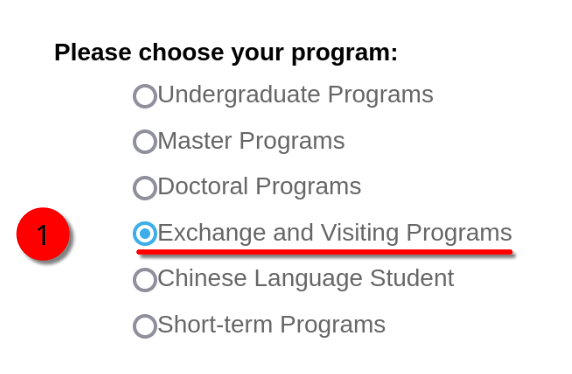
\includegraphics[width=\textwidth]{01_russia/imgs/app_1}
    \end{subfigure}
    \hfill
    \begin{subfigure}[c]{0.49\textwidth}
        \centering
        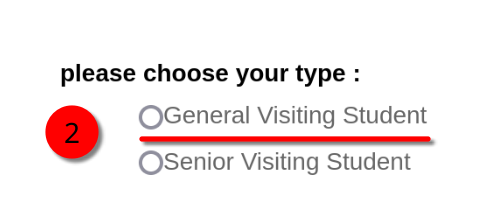
\includegraphics[width=\textwidth]{01_russia/imgs/app_2}
    \end{subfigure}
    \caption{Study Program}
    \label{fig:ru_student_type}
\end{figure}


After, you should specify the Department and Major.
For Department \textcircled{1} and Major \textcircled{2} choose
\textbf{``Computer Science and Technology``}.
Don't forget to specify the English language \textcircled{3}!
Start the search \textcircled{4} and choose appropriate study plan \textcircled{5}.
Additionally, pay attention to application period!
Maybe the application period not started yet.
Fig~\ref{fig:ru_study_plan}


\begin{figure}[htpb]
    \centering
    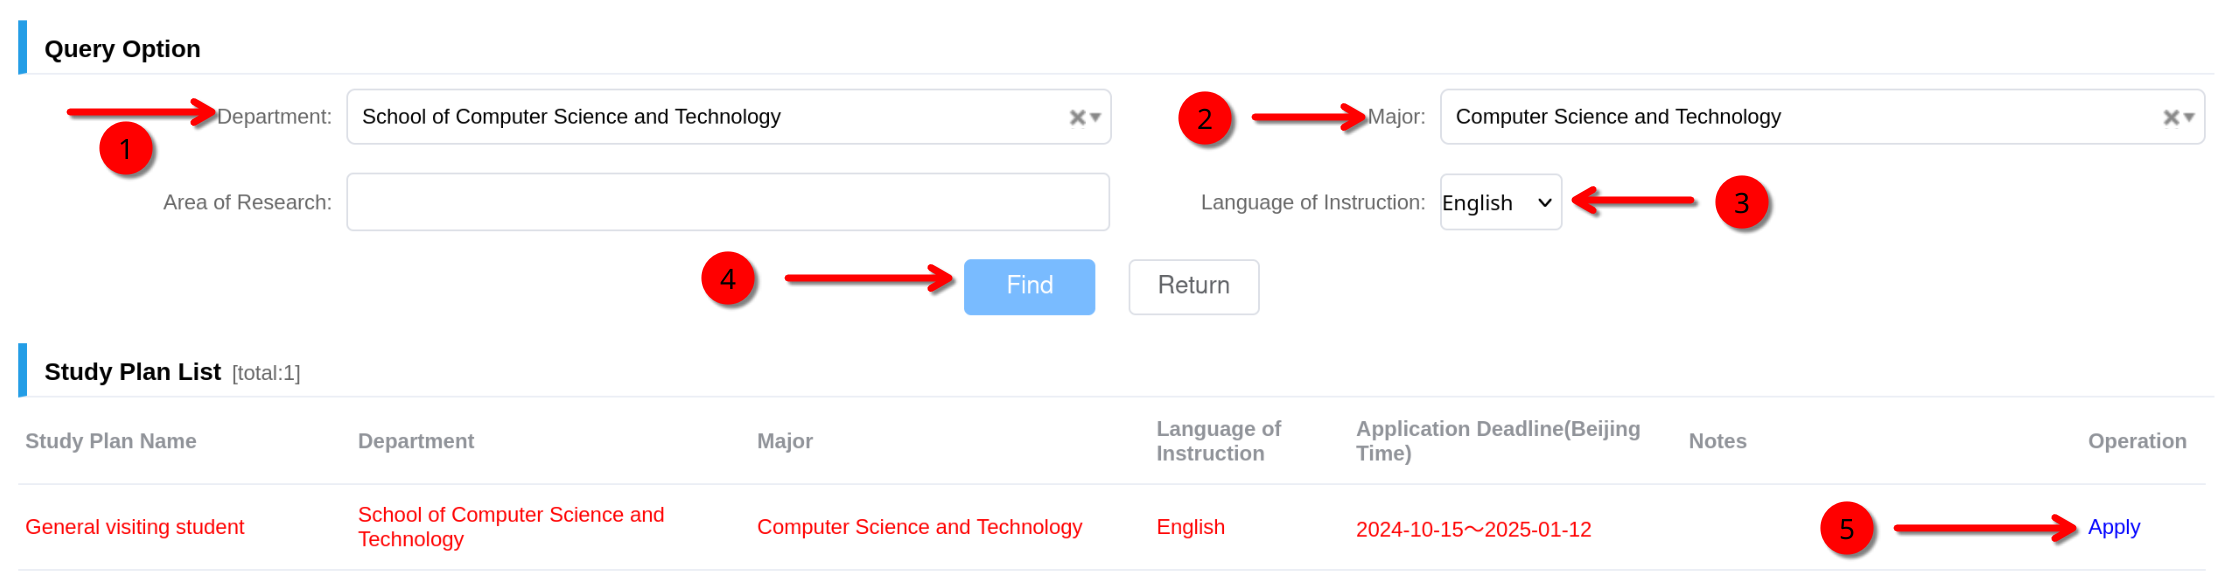
\includegraphics[width=\textwidth]{01_russia/imgs/app_3_study_plan}
    \caption{\centering Study Plans}
    \label{fig:ru_study_plan}
\end{figure}








\section{Personal Information}\label{sec:ru_personal_info}

This section not that hard, but some points should be clarified!
Fig~\ref{fig:ru_pers_info}

\begin{enumerate}
    \item Fill the name and surname according to international passport.
        If you still don't have it, you can check spelling
        \href{https://www.gosuslugi.ru/help/faq/foreign_passport/100359}{HERE}.

    \item \textbf{Highest Level of Education}: Bachelor

    \item \textbf{Final Education Institution}: Innopolis University

    \item \textbf{Occupation}: Student

    \item \textbf{Chinese Name}.
        If you don't have Chinese name yet, leave field blank.
        The Chinese coordinator will give you Chinese names that match the real ones. \\
        \textbf{For example}: Timofei - MoFei, Artur - AnTeng (it may sound not that similar)

    \item \textbf{Employer or Institution Affiliated}: Innopolis University
\end{enumerate}


\begin{figure}[H]
    \centering
    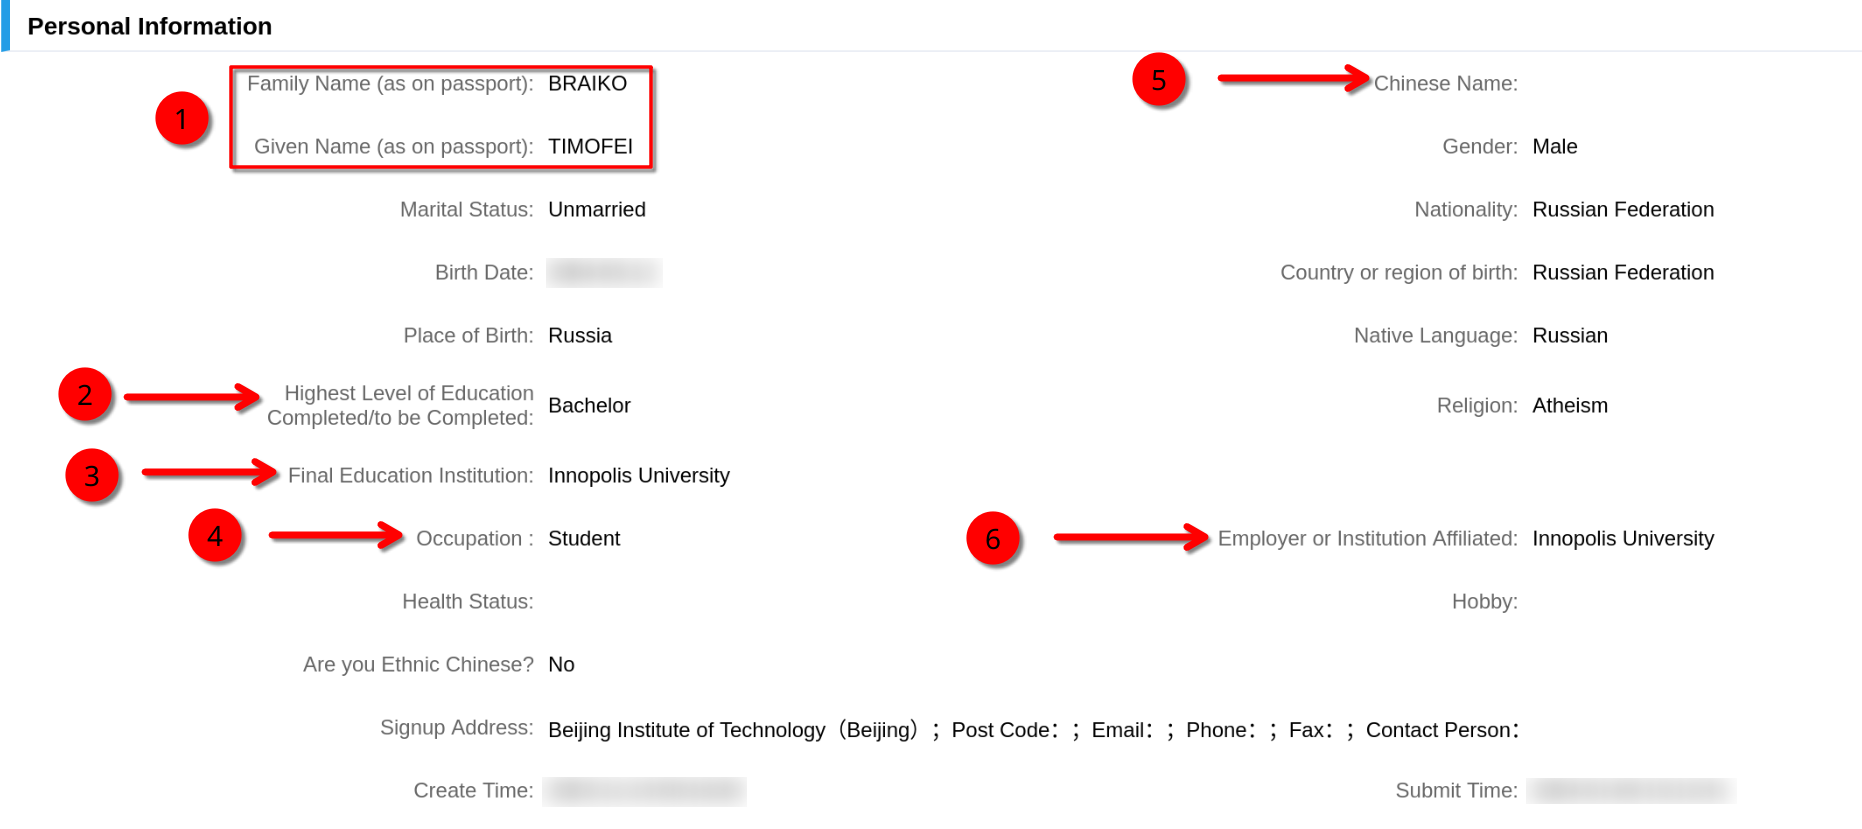
\includegraphics[width=\textwidth]{01_russia/imgs/app_4_personal_info}
    \caption{\centering Personal Information}
    \label{fig:ru_pers_info}
\end{figure}









\section{Passport}\label{sec:ru_passport}

In this section, you fill in your international passport details.
You should get and submit your international passport before application deadline.
Otherwise, write to Innopolis coordinator.
As of 2024, it's Veronika Mezenova (@Nika\_Mezenova)

Regarding field \textbf{Location of Visa Office}.
At the end of 2024, a Chinese visa can be obtained in the following places:

\begin{itemize}
    \item \textbf{Embassy in Russia Federation} - Moscow
    \item \textbf{Consulate in St.Petersburg}
    \item \textbf{Consulate in Yekaterinburg}
    \item \textbf{Consulate in Khabarovsk}
    \item \textbf{Consulate in Vladivostok}
\end{itemize}


\begin{note}
    At the time of writing, a visa cannot be obtained in Kazan.
\end{note}









\section{Language Proficiency}
Enter the exam results.
Please note that if you have passed the IELTS or TOEFL yourself,
they are valid for only two years.
If you passed inner-university exam choose IELTS, as it's based on IELTS exam.
Issue date is printed on certificate Fig~\ref{fig:ru_lang_prof}.


\begin{figure}[H]
    \centering
    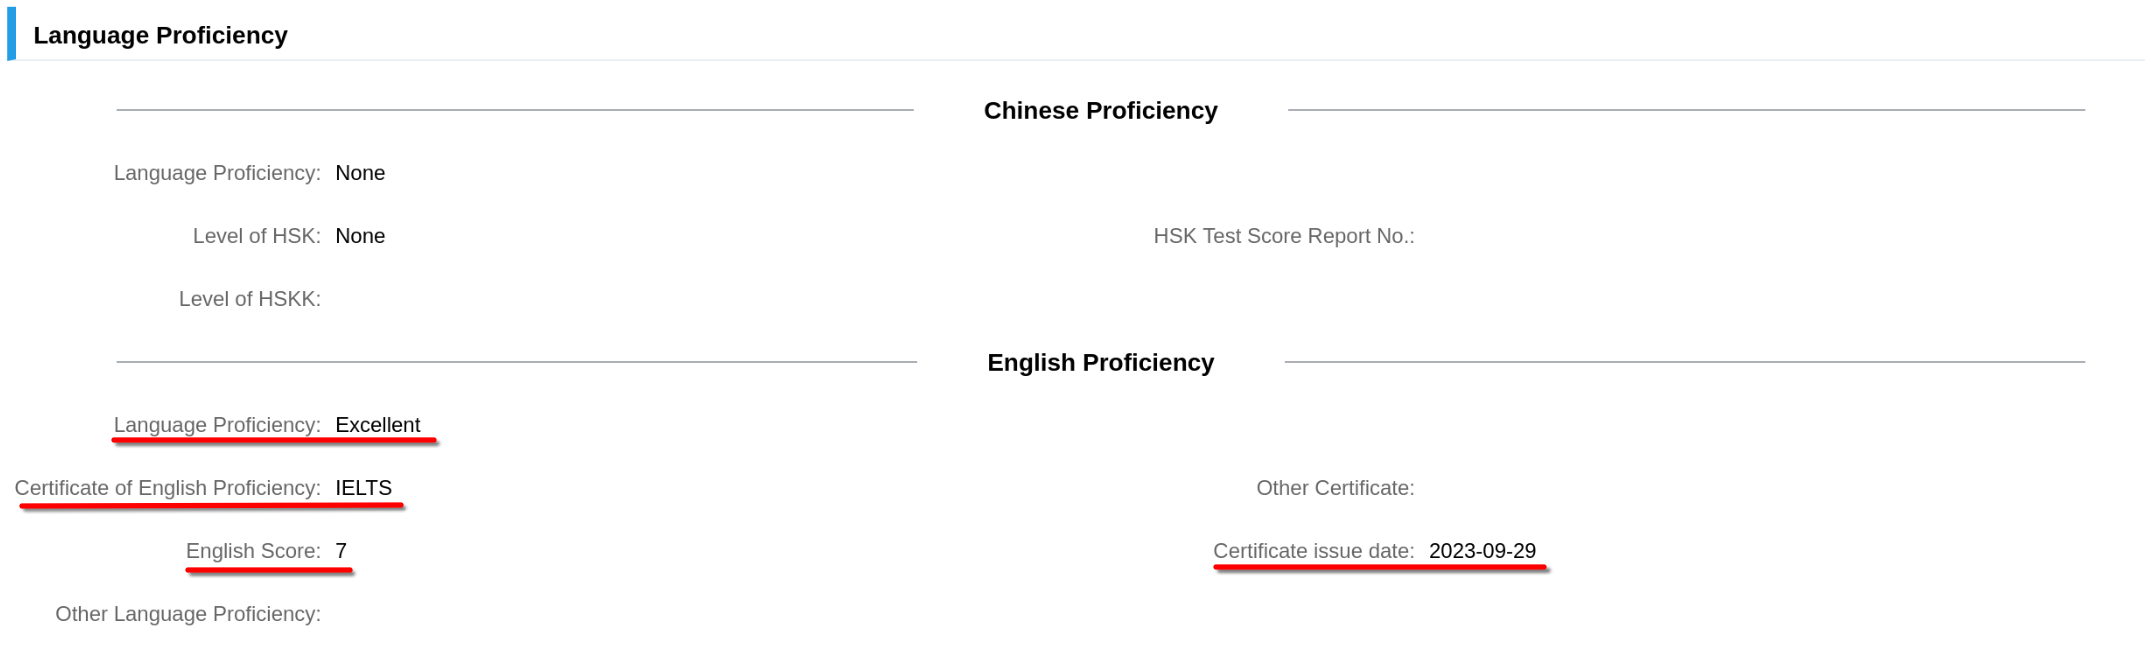
\includegraphics[width=\textwidth]{01_russia/imgs/app_5_language}
    \caption{\centering Language Proficiency}
    \label{fig:ru_lang_prof}
\end{figure}









\section{Recommender}
Specify the head of the department here.
For this moment, he is Petr Zhdanov Fig~\ref{fig:ru_recommender}.

\begin{itemize}
    \item \textbf{Source:} Others - Head of the International Relation Office
    \item \textbf{Name:} Petr Zhdanov
    \item \textbf{Organization:} Autonomous noncommercial organization of higher education ``Innopolis University``.
    \item \textbf{Phone Number:} +7 843 203 92 53
    \item \textbf{Relationship with applicant:} Head of the International Relation Office
    \item \textbf{Email:} pe.zhdanov@innopolis.ru
\end{itemize}


\begin{figure}[H]
    \centering
    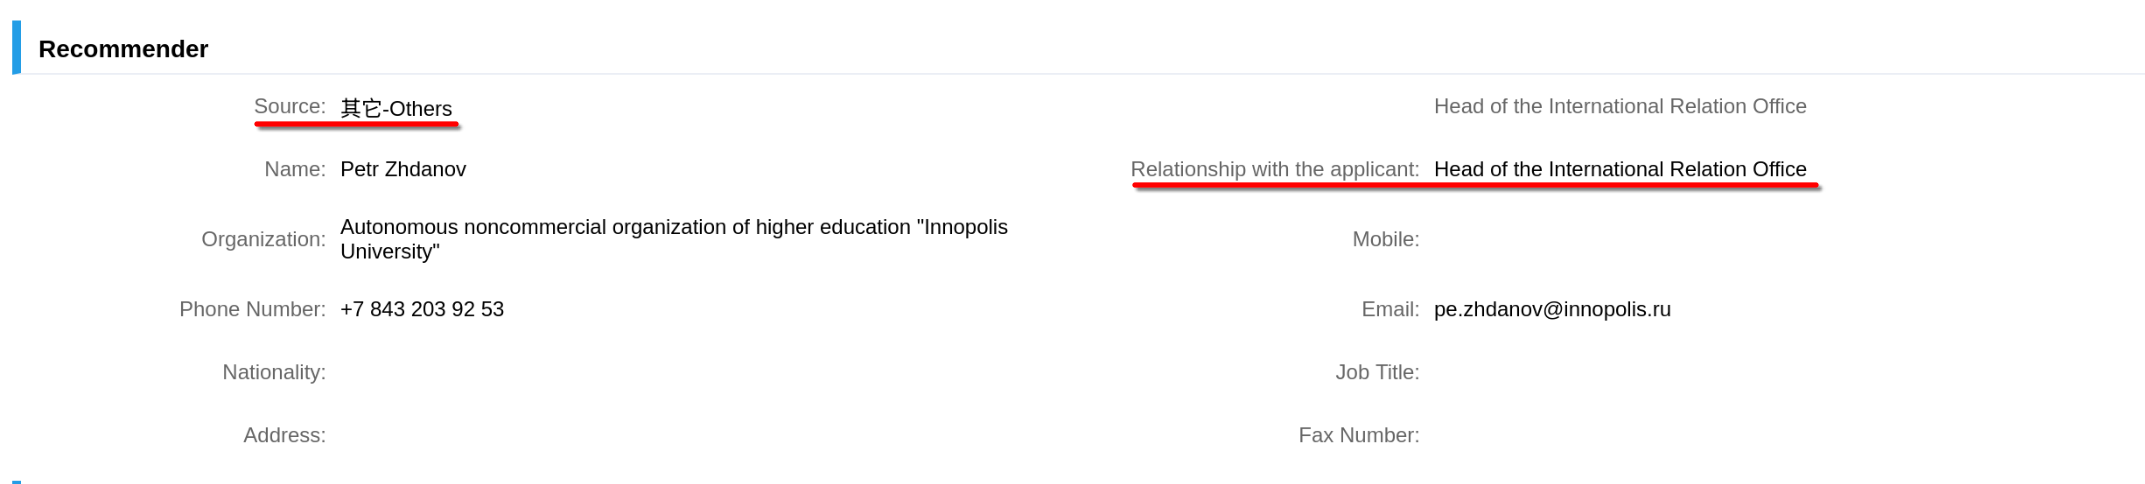
\includegraphics[width=\textwidth]{01_russia/imgs/app_6_recommender}
    \caption{\centering Recommender}
    \label{fig:ru_recommender}
\end{figure}







\section{Educational Background}\label{sec:ru_edu}

This section not so important, if you're bachelor.
Just specify your school.
Below you can see example in Fig~\ref{fig:ru_edu_back}.
Probably not that many details are needed.


\begin{figure}[H]
    \centering
    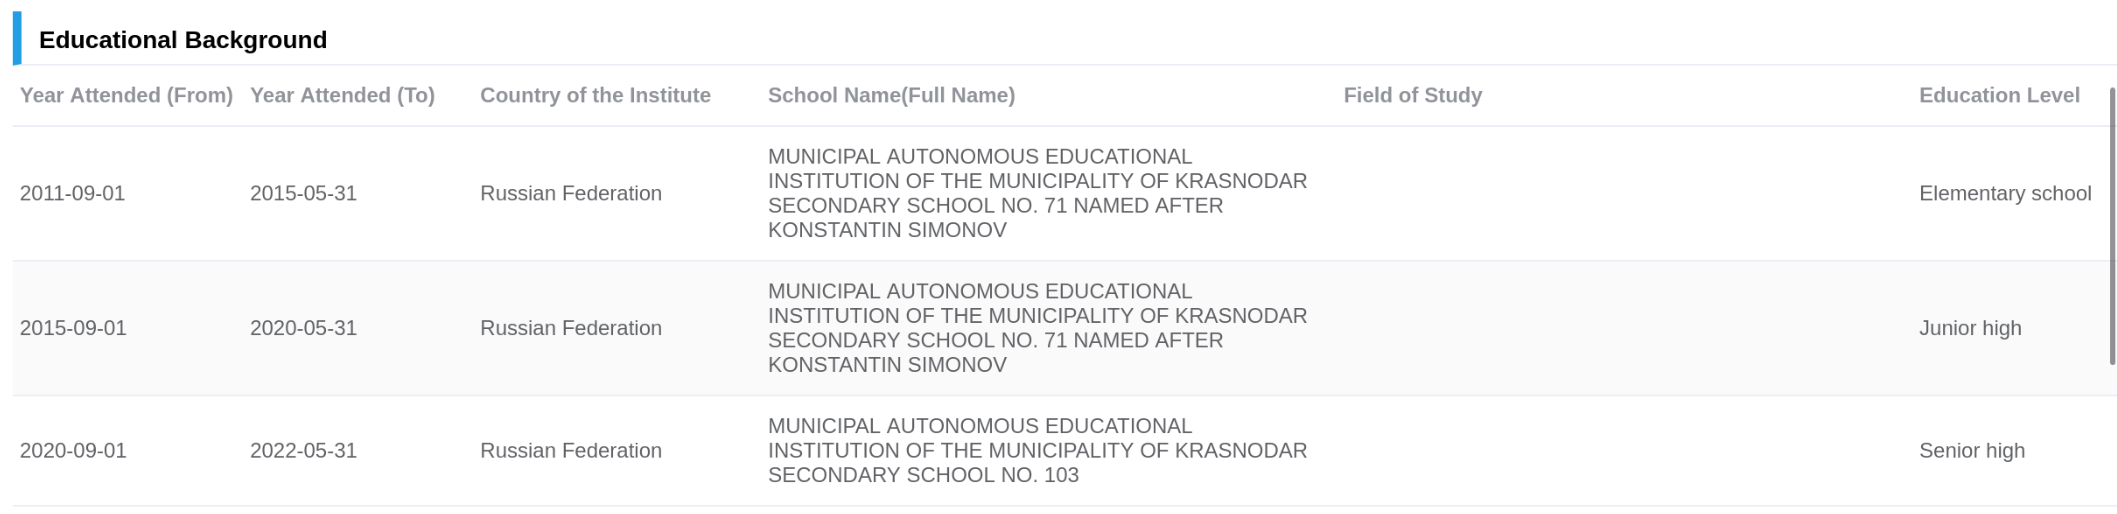
\includegraphics[width=\textwidth]{01_russia/imgs/app_edu_back}
    \caption{\centering Educational Background}
    \label{fig:ru_edu_back}
\end{figure}







\section{Family}\label{sec:ru_family}
Here, specify two relatives (parents)
with their contacts and place of work.


\begin{joke}
The Chinese Party prohibits specifying more than two relatives,
because one family means one child.
Otherwise, the Chinese Party will take away the
cat-wife and a bowl of rice.
\end{joke}





\section{Financial Supporter and Guarantor}\label{sec:ru_fin_supp}
Financial Supporter and Guarantor should be the same person.
This is someone who will financially support you (does not have to live in China).
Basically it's one of the parents.





\section{Addresses}\label{sec:ru_addr}

\begin{itemize}
    \item \textbf{Permanent Address} - address in internal passport
    \item \textbf{Current Postal Address} - Place of current residence.\\
        Innopolis Dorms or Kazan if you live there.
    \item Zip Code for Innopolis: 420500
\end{itemize}







\section{How to collect Admission Notice}\label{sec:ru_adm_not_delivery}

It's the most crucial document you need for exchange program.
Admission notice is enrolment document required to get \textit{Study Visa},
go through border control in China, apply for a bank card and so on.

If you have two options as shown in Fig~\ref{fig:ru_collect_adm_not},
\textbf{it's better to choose deliver option}.
In the end, Admission Notice will be sent by email.
Highly likely this question doesn't affect on anything.
However, better choose delivery option, to not screw up.


\begin{figure}[H]
    \centering
    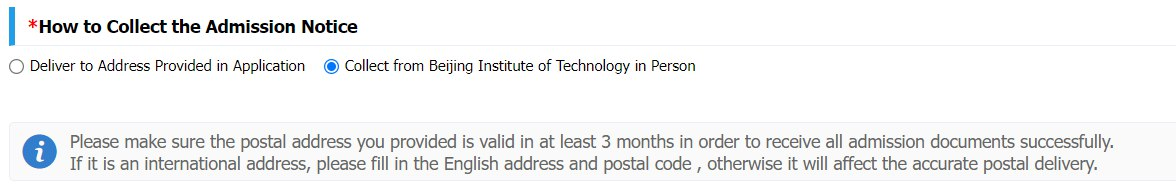
\includegraphics[width=\textwidth]{01_russia/imgs/app_adm_notice}
    \caption{\centering Options to collect Admission Notice}
    \label{fig:ru_collect_adm_not}
\end{figure}






\section{Uploading Documents}\label{sec:ru_upload_docs}

\begin{itemize}
    \item \textbf{Passport} - PDF with main and visa pages

    \item \textbf{Transcripts} - You should have it by this time.
        Otherwise, get it via
    \href{https://my.university.innopolis.ru/profile/edu-certs/create}{Innopolis website}.

    \item \textbf{Proof of Language Proficiency} - Results of English exam.

    \item \textbf{Recommendation Letter} - The same document if you pass inner-exam.
    If you're master student, get it from your supervisor.

    \item \textbf{Physical Examination Records} - See chapter~\ref{...}.

    \item \textbf{Non-Criminal Record} - Chinese guys will do it for you.
\end{itemize}